\chapter{Experimentos e Resultados}
\label{cap:experimentos-resultados}
Este capítulo visa apresentar os testes executados durante o estudo e elaboração deste documento, assim como os resultados alcançados durante a construção. Abordar os principais pilares para a execução  do desenvolvimento e verificação de validação dos testes para alcançar os objetivos do projeto. O desenvolvimento visou trabalhar a partir um escopo menor e ampliar posteriormente.

Para os experimentos de tratamento de imagem foram utilizados três imagens diferentes escolhidas aleatoriamente que cobririam cenários onde há angulação de rosto, presença de cabelo frente a face e fundo com cores próximas a tom de pele para verificar enquadramento e exclusão de regiões sem presença de pele humana. Com essas imagens foram executados alguns testes de dimensionamento e conversão de sistema de cores do RGB para HSV, Lab, YcrCb.

Nos testes iniciais foram utilizadas imagens com apenas um rosto em cada foto, sem padronização de plano de fundo e iluminação. Inicialmente nenhuma formatação nas imagens foi executada, contudo, foi percebido que a identificação de tom de pele dominante nas imagens eram influenciados por regiões da face como olhos e boca e pela presença de pelos e cabelos na imagem. A partir disso, foi iniciado estudos para identificar e contornar a região facial para minimizar as influências indesejadas. 

Foram analisados três classificadores para a identificação facial, sendo elas o Haar Cascade, histogramas e redes neurais convolucionais. As três opções são amplamente utilizadas para na área de reconhecimento facial. Neste caso, foi optado por utilizar o classificador Haar Cascade pela facilidade de utilização e de identificação de diferentes características que planejou-se eliminar durante a manipulação das imagens, com pouca necessidade de codificação.Neste caso, não foi considerado relevante o tempo de processamento das imagens e não foi avaliado os resultados de precisão que os modelos obteriam. Baseado no resultado do classificador, escolheu-se recortar as imagens onde o algoritmo identificou e contornado a face, retornando uma imagem com menos influência de objetos e cabelo. Isso melhorou a percepção de coloração dominante na paleta resultante.

Utilizando com base o estudo o \cite{Automatic_Skin_Tone_Extraction_for_Visagism_Applications} e a Tabela \ref{table:Tabela_comparativa_sistemas_de_cores} optou-se por escolher um sistema de cor com bom desempenho para ser utilizado, sendo o escolhido o padrão HSV. O HSV é um sistema de cor utilizado para identificação de cores e considerando o estudo obteve os mesmo resultados de previsão comparado ao sistema YCrCb. Contudo, preferiu-se utilizar o sistema HSV pela sua simplicidade já que o componente de saturação (H) possui a informação de coloração absoluta simplificando possíveis ajustes, em contrapartida, ao formato YCrCb que se faz necessário o controle de duas variáveis (Cr e Cb).

\begin{figure}[h]
\centering
\caption{Etapas de desenvolvimento}
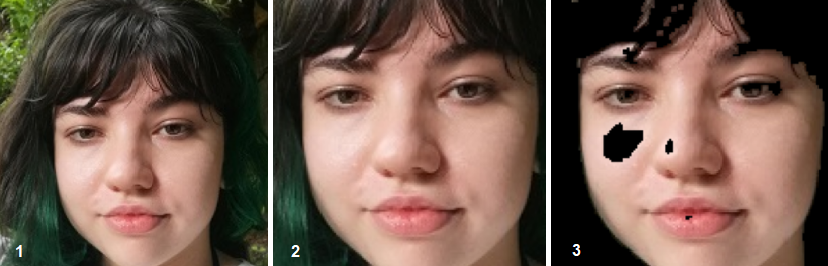
\includegraphics{Template_Latex_TCC-UNIFTEC/_lib/imagens/vittoriatestes.png}

\label{fig:x Etapas_de_teste}
\centering{\Fonte{Autor}}
\end{figure}

Para a identificação de tom de pele 

Para a categorização foi utilizados 

Para a validação da identificação de pele foram utilizadas imagens 

